\section{Video Prediction for Control}
\label{sec:model}

\begin{figure}[t]
	\centering
	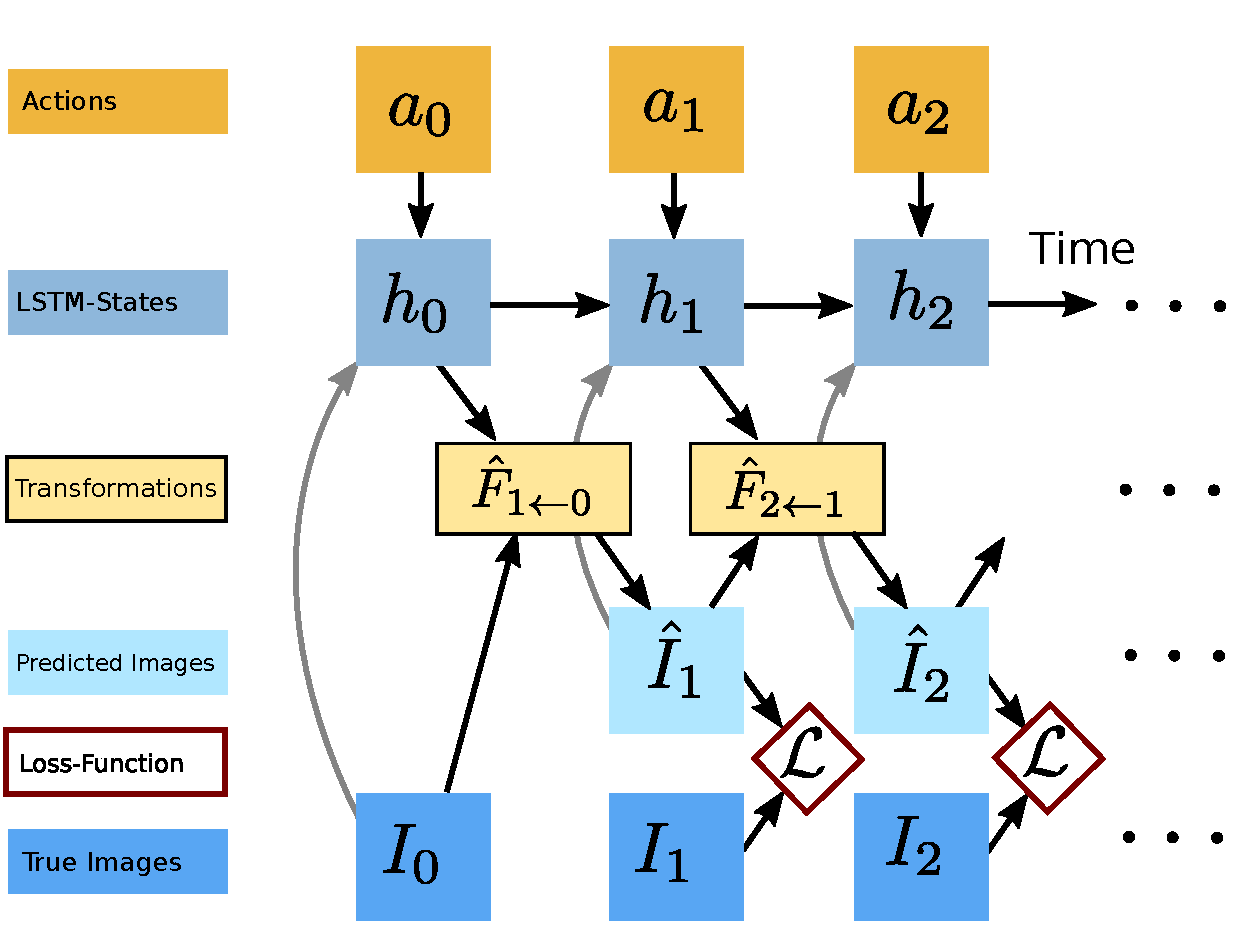
\includegraphics[width=0.8\columnwidth]{images_general/prediction_model.pdf}
	\caption{\small{Computation graph of the video-prediction model. Time goes from left to right, $a_t$ are the actions, $h_t$ are the hidden states in the recurrent neural network, $\hat{F}_{t+1 \leftarrow t}$ is a 2D-warping field, $I_t$ are real images, and $\hat{I}_t$ are predicted images, $\mathcal{L}$ is a pairwise training-loss.}}   
	\label{fig:prediction_model}
\end{figure}

In visual MPC, we use a transformation-based video prediction architecture, first proposed by Finn et al. \cite{finn_nips}. The advantage of using transformation-based models over a model that directly generates pixels is two-fold: (1) prediction is easier, since the appearance of objects and the background scene can be reused from previous frames and (2) the transformations can be leveraged to obtain predictions about where pixels will move, a property that is used in several of our planning cost function formulations. The model, which is implemented as a recurrent neural network (RNN) $g_{\theta}$ parameterized by $\theta$, has a hidden state $h_t$ and takes in a previous image and an action at each step of the rollout.  Future images $\hat{I}_{t+1}$ are generated by warping the previous generated image $\hat{I}_t$ or the previous true image $I_t$, when available, according to a 2-dimensional flow field $\hat{F}_{t+1 \leftarrow t}$. A simplified illustration of model's structure is given in figure \ref{fig:prediction_model}. It is also summarized in the following two equations:
\begin{align}
[h_{t+1}, \hat{F}_{t+1 \leftarrow t}] 	&= g_{\theta}(a_t, h_t, I_t) \\
\hat{I}_{t+1} 							&= \hat{F}_{t+1 \leftarrow t} \diamond  \hat{I}_t 
\label{simple_dna}
\end{align}
Here, the bilinear sampling operator $\diamond$ interpolates the pixel values bilinearly with respect to a location $(x,y)$ and its four neighbouring pixels in the image, similar to \cite{zhou2016view}. Note that, as shown in figure \ref{fig:prediction_model}, at the first time-step the real image is transformed, whereas at later timesteps previously generated images are transformed in order to generate multi-frame predictions. The model is trained with gradient descent on a $\ell_2$ image reconstruction loss, denoted by $\mathcal{L}$ in figure \ref{fig:prediction_model}.
\begin{figure}[t]
    \centering
    \includegraphics[width=\columnwidth]{images_sna/occlusionaware/architecture_2.pdf}
    \caption{\small{Forward pass through the recurrent SNA model. The red arrow indicates where the image from the first time step $I_0$ is concatenated with the transformed images $\hat{F}_{t+1 \leftarrow t} \diamond  \hat{I}_t $ multiplying each channel with a separate mask to produce the predicted frame for step $t+1$.}}      \label{fig:occlusion_model}
\end{figure}
A forward pass of the RNN is illustrated in figure \ref{fig:occlusion_model}. We use a series of stacked convolutional LSTMs and standard convolutional layers interleaved with average-pooling and upsampling layers. The result of this computation is the 2 dimensional flow-field $\hat{F}_{t+1 \leftarrow t}$ which is used to transform a current image $I_t$ or $\hat{I}_t$. \edit{More details on the architecture are provided in the appendix. \todo{add appendix}}

\noindent \textbf{Predicting motion of individual pixels}: 
When using visual MPC with a cost-function based on start and goal pixel positions, we require a model that can effectively predict the 2D motion of the user-selected start pixels $\pixel_0^{(1)}, \dots, \pixel_0^{(P)}$ up to $T$ steps into the future\footnote{Note that when using a classifier-based cost function, we do not require the model to output transformations.}.
More details about the cost functions are provided in section \ref{sec:cost}. Since the model we employ is transformation-based, this motion prediction capability emerges automatically, and therefore no external pixel motion supervision is required. To predict the future positions of the designated pixel $d$, the same transformations used to transform the images are applied to the distribution over designated pixel locations. The warping transformation $\hat{F}_{t+1 \leftarrow t}$ can be interpreted as a stochastic transition operator allowing us to make probabilistic predictions about future locations of individual pixels:
\begin{equation}
\hat{P}_{t+1} = \hat{F}_{t+1 \leftarrow t} \diamond  \hat{P}_t
\label{eqn:prob_forward}
\end{equation}
Here, $P_t$ is a distribution over image locations which has the same spatial dimension as the image. For simplicity in notation, we will use a single designated pixel moving forward, but using multiple is straightforward. At the first time step, the distribution $\hat{P}_0$ is defined as 1 at the position of the user-selected designated pixel and zero elsewhere. The distribution $\hat{P}_{t+1}$ is normalized at each prediction step.

Since this basic model, referred to as dynamic neural advection (DNA), predicts images only based on the previous image, it is unable to recover shapes (e.g., objects) after they have been occluded, for example by the robot arm. Hence, this model is only suitable for planning motions where the user-selected pixels are not occluded during the manipulation, limiting its use in cluttered environments or with multiple selected pixels. In the next section, we introduce an enhanced model, which lifts this limitation by employing temporal skip connections. 

\noindent \textbf{Skip connection neural advection model}
To enable effective tracking of objects through occlusions, we can add temporal skip connections to the model: we now transform pixels not only from the previously generated image $\hat{I}_t$, but from all previous images $\hat{I}_1,...\hat{I}_{t}$, including the context image $I_0$, which is a real image. All these transformed images can be combined to a form the predicted image $\hat{I}_{t+1}$ by taking a weighted sum over all transformed images, where the weights are given by masks $\mathbf{M}_t$ with the same size as the image and a single channel:
\begin{equation}
\hat{I}_{t+1} =  \mathbf{M}_{0} (\hat{F}_{t+1 \leftarrow 0} \diamond I_t) +  \sum_{j=1}^{\tau} \mathbf{M}_{j} (\hat{F}_{t+1 \leftarrow j} \diamond  \hat{I}_j).
\end{equation}
We refer to this model as the \emph{skip connection neural advection model (SNA)}, since it handles occlusions by using temporal skip connections such that when a pixel is occluded, e.g., by the robot arm or by another object, it can still reappear later in the sequence.
Transforming from all previous images comes with increased computational cost, since the number of masks and transformations scales with the number of time-steps $\tau$. However, we found that in practice a greatly simplified version of this model, where transformations are applied only to the previous image and the \emph{first image} of the sequence $I_0$, works equally well. Moreover we found that transforming the first image of the sequence is not necessary, as the model uses its pixels primarily to generate the image background. Therefore, we can use the first image directly, without transformation. More details can be found in the appendix \ref{sec:skipcon} and \cite{sna}.